\documentclass[english,notitlepage]{revtex4-1}  

\usepackage[utf8]{inputenc}
\usepackage{physics,amssymb}  
\include{amsmath}
\usepackage{graphicx}         
\usepackage{xcolor}           
\usepackage{hyperref}         
\usepackage{listings}         
\usepackage{subfigure}        
\usepackage{float}
\usepackage{algorithm}
\usepackage[noend]{algpseudocode}
\usepackage{subfigure}
\usepackage{tikz}
\usetikzlibrary{quantikz}

\hypersetup{ 
	colorlinks,
	linkcolor={red!50!black},
	citecolor={blue!50!black},
	urlcolor={blue!80!black}}


\begin{document}
	
	\title{FYS3150 Project 1}      
	\author{Andreas Isene}         
	\date{\today}                             
	\noaffiliation                          
	
	
	\maketitle 
	
	https://github.com/andris96/FYS3150
		 
	\section*{Problem 1}
	This can be done by simply differentiating twice like so:
	\[ u(x) = 1-(1-e^{-10})x-e^{-10x} = 1 - x + e^{-10}x-e^{-10x}\]
	
	\[\frac{du}{dx} =-1+e^{-10}+10e^{-10x}\]
	
	\[\frac{d^2u}{dx^2} = -100e^{-10x}\rightarrow -\frac{d^2u}{dx^2} = 100e^{-10x}\]
	
	\section*{Problem 2}
	
	figure \ref{fig:data_plott} is a plot of the analytical solution to the particular case of the one-dimensional Poisson equation. Code is available on GitHub.
	
	\begin{figure}[h!]
		\centering 
		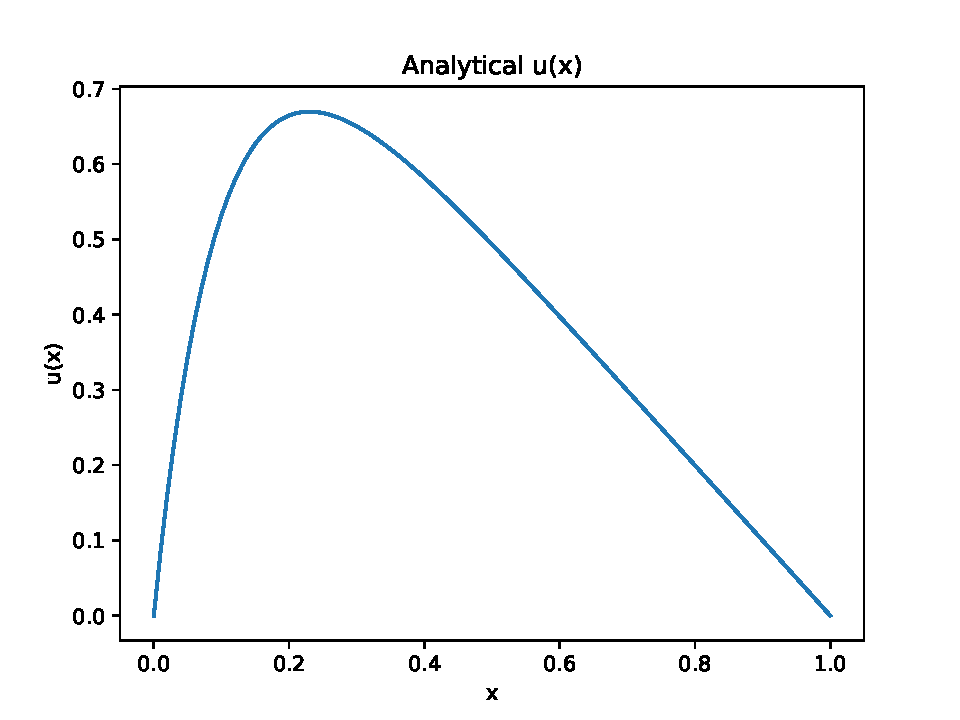
\includegraphics[scale=0.55]{data_plott.pdf}
		\caption{Plot of the analytical solution u(x)}
		\label{fig:data_plott}
	\end{figure}

	\section*{Problem 3}
	From the taylor expansion of $u(x+h)$ and $u(x-h)$ we can derrive an expression for $u''$.
	
	
		\[u(x+h) = u(x) + u'(x)h + 1/2 u''(x)h^2 + \frac{1}{6}u''(x)^3 + O(h^4)\]
		
		\[u(x-h) = u(x) - u'(x)h + 1/2 u''(x)h^2 - \frac{1}{6}u''(x)^3 + O(h^4)\]
		
	Adding them together cancels every other term, with some algebra we end up with the following expression.
	
	
		$$-u''(x) =\frac{-u(x+h)+2u(x)-u(x-h)}{h^2} +O(h^2) = f(x)$$
	

	by defining $v(x_i) = v_i$ as an approximation of $u(x)$ we can remove $O(h^2)$ and finally express the discretized version.
	
	\begin{equation}\label{eq1}
	\frac{-v_{i-1} + 2v_{i} - v_{i+1}}{h^2} \approx f(x_i) = f_i
	\end{equation}

	\section*{problem 4}
	Moving over the $h^2$ in Eq. \ref{eq1} gives the equation:
	
	$$ -v_{i-1} + 2v_{i} - v_{i+1} = h^2f_i$$
	
	If we iterate trough each element from say $i  \in [0,5]$ we can see a pattern.
	
	$$ -v_0 + 2v_1 -v_2 = h^2f_1 $$ 
	$$ -v_1 + 2v_2 -v_3 = h^2f_2 $$ 
	$$ -v_2 + 2v_3 -v_4 = h^2f_3 $$ 
	$$ -v_3 + 2v_4 -v_5 = h^2f_4 $$ 
	
	Since the boundaries are known we can move over $v_1$ and $v_5$ to the other side and express everything in terms of matrices.
	
	\[
	\begin{pmatrix}
		2 & -1 & 0 & 0\\
		-1 & 2 & -1 & 0\\
		0 & -1 & 2 & -1\\
		0 & 0 & -1 & 2
	\end{pmatrix}
	\begin{pmatrix}
		v_1\\v_2\\v_3\\v_4
	\end{pmatrix}
	=
 	\begin{pmatrix}
 		h^2f_1+v_0\\h^2f_2\\h^2f_3\\h^2f_4+v_5
 	\end{pmatrix}
 	=
 	\begin{pmatrix}
 		g_1\\g_2\\g_3\\g_4
 	\end{pmatrix}
	\] 
	
	This looks much like the matrix equation given. The different $g_i$ are given by $h^2f_i$ except at the boundaries where we ad $v_0 or v_5$. 
	
	\section*{problem 5}
	\textbf{a)} 
	$$n = m-2$$
	\textbf{b)} 
	The vector $\overrightarrow{v}$ excludes the boundary points. A complete solution would include the boundaries, which means that two more points would have to be added.
	
	\section*{problem 6}
	\textbf{a)}
	The equation can be solved with forward- followed by backward substitution, an algorithm for each method is shown in \ref{forward} and \ref{backwardward}. The $a_i$, $b_i$ and $c_i$ are corresponding to elements in the subdiagonal, diagonal and superdiagonal respectively. $\tilde{b}$ and $\tilde{g}$ are new variables that needs to be defined in order to solve
	\begin{algorithm}[H]
		\caption{Forward substitution}\label{forward}
		\begin{algorithmic}
			\State $\tilde{b}_1 = b_1$
			\For{$i = 2, 3, ..., n$}
			\State $\tilde{b}_i = b_i - a_ic_i/\tilde{b}_{i-1}$
			\EndFor
			\State $\tilde{g}_1 = g_1$
			\For{$i = 2, 3, ..., n$}
			\State $\tilde{g}_i = g_i - a_i\tilde{g}_i/\tilde{b}_{i-1}$
			\EndFor
		\end{algorithmic}
	\end{algorithm}

	\begin{algorithm}[H]
		\caption{backward substitution}\label{backwardward}
		\begin{algorithmic}
			\State $v_n = \tilde{g}_n/\tilde{b}_n$
			\For{$i = n-1, n-2, ..., 1$}
			\State $v_i = (\tilde{g}_i - c_iv_{i+1})/\tilde{b}_{i}$
			\EndFor	
		\end{algorithmic}
	\end{algorithm}	

	\textbf{b)} For each iteration in the first algorithm we do a floating operation 3 times in the first loop and 3 times in the second loop, since there are no calculations for i = 1, we get 3n-1 FLOPs twice, which means 6n-2 $\approx$ 6n FLOPs. In the second algorithm there is no calculation for i = n, giving us a total of 3n-1 $\approx$ 3n FLOPs. This amounts to a total of approximately 9n FLOPs to solve the equation.
	
	
	\section*{problem 7}
	\textbf{a)} Program can be found in the GitHub link.
	
	\textbf{b)} 
	
	Figure \ref{fig:v1_plott}, \ref{fig:v2_plott} and \ref{fig:v3_plott} are supposed to be the numerical solutions with increasing n. We can see that there must be some mistakes in the program, since the value of v becomes smaller with increasing n, which is not supposed to happen. It should increase in precision and become more like u as n increases. This might be because of problems with indexing. It started to become very confusing the when i tried to use $\overrightarrow{v}^*$ instead of $\overrightarrow{v}$. There could also be a mistake in the calculations around the boundaries. If the first calculation is wrong then all subsequent calculations will also be wrong, making the problem worse. The shape of the curve is not too far off from the analytical curve, making me think that some small adjustments could result in a good approximation. There could also be some mistake in the algorithm, of course. 
	
	\begin{figure}[H]
		\centering
		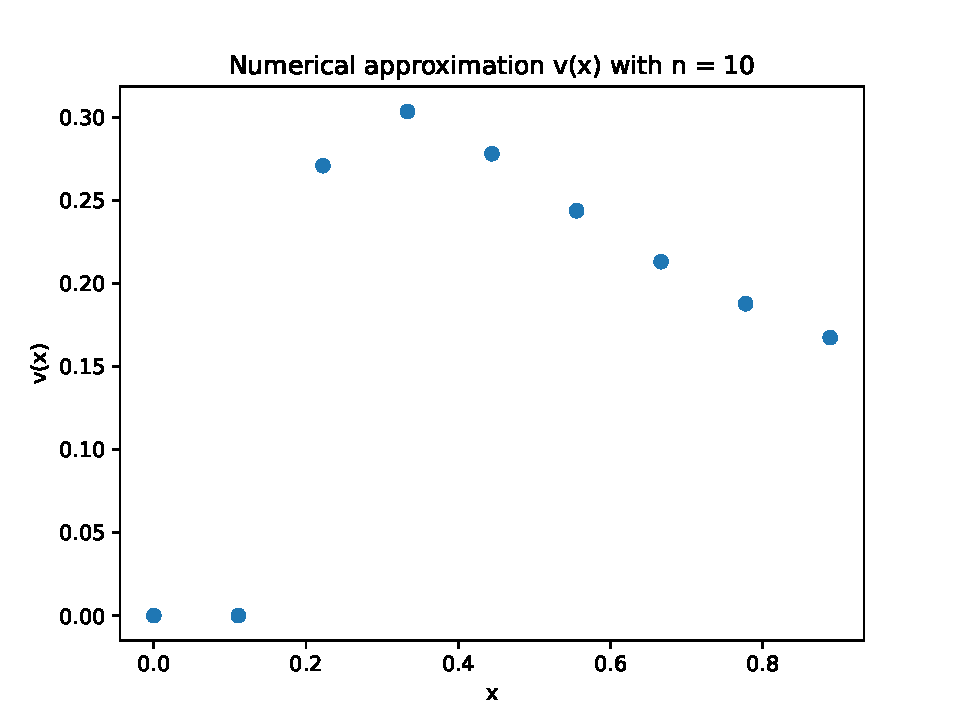
\includegraphics[scale=0.55]{v1_plot.pdf}
		\caption{Plot of the numerical solution v(x) with n = 10}
		\label{fig:v1_plott}
	\end{figure}

	\begin{figure}[H]
		\centering
		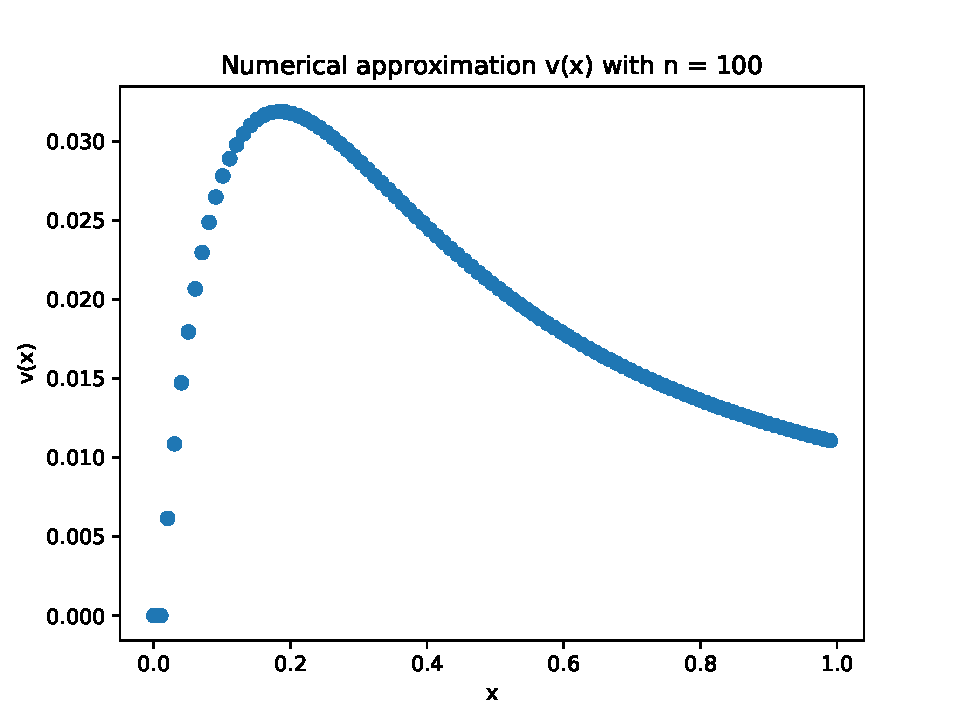
\includegraphics[scale=0.55]{v2_plot.pdf}
		\caption{Plot of the numerical solution v(x) with n = 100}
		\label{fig:v2_plott}
	\end{figure}

	\begin{figure}[H]
		\centering
		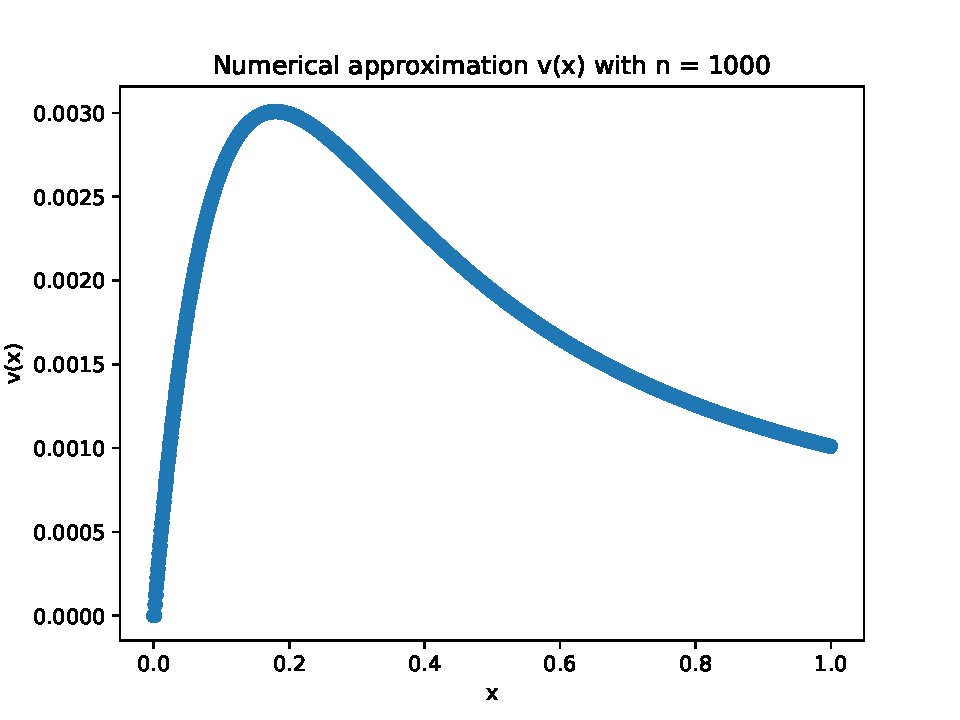
\includegraphics[scale=0.55]{v3_plot.pdf}
		\caption{Plot of the numerical solution v(x) with n = 1000}
		\label{fig:v3_plott}
	\end{figure}

	\section*{problem 8}
	as I am running out of time, and the results from problem 7 would make it hard to interpret the plots in problem 8, i have decided to move on to problem 9.
	
	\section*{problem 9}
	
	\textbf{a)} With the specialized algorithm, we can exclude multiple operations, making the FLOP count much smaller. The $a_i$, $b_i$ and $c_i$ are all the same for every i, resulting in algorithms \ref{forward2} and \ref{backwardward2}.
	
	\begin{algorithm}[H]
		\caption{Forward substitution}\label{forward2}
		\begin{algorithmic}
			\State $\tilde{b}_1 = 2$
			\For{$i = 2, 3, ..., n$}
			\State $\tilde{b}_i = 2-1/\tilde{b}_{i-1}$
			\EndFor
			\State $\tilde{g}_1 = g_1$
			\For{$i = 2, 3, ..., n$}
			\State $\tilde{g}_i = g_i +\tilde{g}_i/\tilde{b}_{i-1}$
			\EndFor
		\end{algorithmic}
	\end{algorithm}
	
	\begin{algorithm}[H]
		\caption{backward substitution}\label{backwardward2}
		\begin{algorithmic}
			\State $v_n = \tilde{g}_n/\tilde{b}_n$
			\For{$i = n-1, n-2, ..., 1$}
			\State $v_i = (\tilde{g}_i + v_{i+1})/\tilde{b}_{i}$
			\EndFor	
		\end{algorithmic}
	\end{algorithm}	

	\textbf{b)} In each for loop there are now 2 FLOPs per iteration, which gives around 6n FLOPs in total.

	
	
		
		

	
\end{document}
